%%%%%%
%	Præamble
%%%%%%

\documentclass{report}

%%%%%%
%	Præambel
%%%%%%

%\documentclass{report}

%	Pakker

\usepackage[utf8]{inputenc}
\usepackage[T1]{fontenc}
\usepackage{graphicx}
\usepackage[cc]{titlepic}
\usepackage{verbatim}
\usepackage{lipsum}
\usepackage{rotating}
\usepackage{fancyvrb}
\usepackage{titling}
\usepackage{listings}
\usepackage{hyperref}
\usepackage[dvipsnames,table]{xcolor}
\usepackage{pdfpages}
\usepackage{float}
\usepackage[danish]{babel}
\usepackage{datetime}
\usepackage{tabularx}
\usepackage{newclude}
\usepackage{tikz}
\usepackage{tablefootnote}

%	Bibloteker

\usetikzlibrary{shapes, arrows}

%	Opsætning

\graphicspath{{./billeder/}}

%	kommandoer

\newcommand{\pic}[2][png]{
	\includegraphics[width=\textwidth]{./#2.#1}
}

\newcommand{\fragCom}[1]{
	\textcolor{LimeGreen}{\texttt{\textbf{#1}}}
}

\newcommand{\logDay}[2][2]{\section*{\formatdate{#2}{#1}{2023}}}

%environmental setup

\lstset{
	breaklines=true,
	breakatwhitespace=true,
	texcl=true,
	extendedchars=false,
	frame=single,
	tabsize=2
}

\lstset{literate=%
	{æ}{{\ae}}1
	{ø}{{\o}}1
	{å}{{\aa}}1
}

%	titel and Aarhus Tech titlecard
\newcommand{\writer}{Sune Koch Rønnow}
%\newcommand{\advisor}{Rasmus Ladefoged Wolffram \& Kenneth Løvgren}
\newcommand{\advisorTwo}{Rasmus Ladefoged Wolffram}
\newcommand{\advisorOne}{Kenneth Løvgren}
\newcommand{\advisor}{\advisorOne{} \& \advisorTwo{}}
\newcommand{\projectName}{ObliGentle}
\newcommand{\reportType}{unavngivenreport}
\newcommand{\reportName}{
	\projectName{}: \reportType{}
}

\newcommand{\subtitle}[1]{%
	\posttitle{%
		\par\end{center}
	\begin{center}\large#1\end{center}
	\vskip0.5em}%
}

\title{\reportName{}}
\subtitle{Svendeprøve ved \\ \advisorOne{} \\ \& \\ \advisorTwo{} \\ \vspace{0.75\baselineskip} Aarhus Tech}
\author{\writer{} \\ sune@kochroennow.dk}
\date{\today}
%\date{\formatdate{6}{10}{2023}}

\newcommand{\makeTechTitlecard}{
	\chapter*{Titelblad}
	\begin{table}[h]
	\center
	\begin{tabularx}{\textwidth}{p{.3\linewidth} X}
	\textbf{Deltagere}		&	\writer{}												\\
	\textbf{Projektnavn} 	&	\projectName{}											\\
	\textbf{Skole}			&	Aarhus Tech \newline{} Hasselager Allé 2, 8260 Viby J	    \\
	\textbf{Projektperiode}	&	\formatdate{13}{11}{2023} - \formatdate{15}{12}{2023}		\\
	\textbf{Afleveringsdato}&	\formatdate{8}{12}{2023}									\\
	\textbf{Vejleder}		&	\advisor{}												\\
	\end{tabularx}
	\end{table}
	\section*{Underskrifter}
	\vspace{3\baselineskip}
	\hrule
	\noindent\small \writer{} \null\hfill Dato\\
	\vspace{2\baselineskip}
	\hrule
	\noindent\small \advisorOne{} \null\hfill Dato\\
	\vspace{2\baselineskip}
	\hrule
	\noindent\small \advisorTwo{} \null\hfill Dato\\
}

% tikz setup

\tikzstyle{terminator} = [rectangle, draw, text centered, rounded corners, minimum height=2em, fill=Magenta!40]
\tikzstyle{process} = [rectangle, draw, text centered, minimum height=2em, fill=Blue!40]
\tikzstyle{positive} = [rectangle, draw, text centered, minimum height=2em, fill=Green!40]
\tikzstyle{negative} = [rectangle, draw, text centered, minimum height=2em, fill=Red!40]
\tikzstyle{decision} = [diamond, draw, text centered, minimum height=2em, fill=Yellow!40]
\tikzstyle{input}=[trapezium, draw, text centered, trapezium left angle=60, trapezium right angle=120, minimum height=2em, fill=Cyan!40]
\tikzstyle{connector} = [draw, -latex']
\tikzstyle{semiConnector} = [draw, -latex',dotted]

% individuel report konfiguration
\renewcommand{\reportType}{Produktrapport}

%%%%%%
%	Indhold
%%%%%%

\begin{document}

\maketitle
\makeTechTitlecard
\tableofcontents

\chapter{Læsevejledning}

I forbindelse med svendeprøven er vi blevet pålagt at aflevere 2 rapporter, en om projektets proces og en om dets produkt. Dette er produktrapporten og fokuserer på gennemgang af brugen af projektet.\par{}
Brugervejledningen er skrevet, således at den ikke kræver nogen særlig teknisk viden.
Den tekniske dokumentation forudsætter en teknisk viden svarende til en færdiguddannet datateknikker.\par{}
Kravspecifikationen er skrevet med henblik  på at være læselig for alle, men da den inkluderer fagudtryk, er den fulde forståelse er muligvis ikke tilgængelig for alle.

\chapter{Kravsspecifikation}
\label{kravspec}

\projectName{} er en opgave-organiserings-/kalenderapplikation, som har til formål at hjælpe brugeren med at organisere deres hverdag ved at give brugeren en positiv oplevelse med, hvad brugeren faktisk når og mindre skyldfølelse med hvad brugeren ikke når. \projectName{} forsøger at opnå dette ved behandle opgaver forskelligt og deler\footnote{I hvert fald i første omgang} op i 3 slags opgaver. Aftaler: Opgaver som skal være færdige til eller før et bestemt tidspunkt, Projekter: selvvalgte opgaver med fokus på fremskridt i stedet for færdiggørelse, 3) Tjanser: Gentagende opgaver.

\subsection{Funktionalitet}

\projectName{} er i sin essens 3 klasser/lister, som hver rummer opgaver. De forskellige klasser/lister har forskellige regler. Endvidere har de også følgende funktioner:
\begin{itemize}
\item uulighed for at tilføje nye opgaver
\item mulighed for at vise udvalgte opgaver
\item \textit{crossplatform accessibility}
\item mulighed for at let at kunne tilføje ekstra funktioner til programmet\footnote{Altså programmet er skrevet modulært; skal ikke forstås som om brugere selv kan ændre programmet}
\item mulighed for brugerne kan bruge \textit{two factor authentication}
\end{itemize}

\subsection{Begrænsninger}

\projectName{} bliver ikke tilgængeligt på \textit{IOS}-enheder.

Selvom \projectName{} vil være tilgængeligt online, vil de juridiske sider i forhold til GDPR og databeskyttelse ikke være en prioritet at færdiggør i en sådan grad, at det frit kan afbenyttes.

\projectName{} er ikke baseret på forskning, men på personlige præferencer.

Sidst men ikke mindst bliver \projectName{} kun en prototype og ikke alle funktioner vil være færdigudviklet.

\projectName{} designes til at kunne videreudvikles til at kunne overkomme alle de begrænsninger, men det kan ikke nås under svendeprøven.

\subsection{Testkonditioner}

\begin{itemize}
\item API'en skal kunne tilgås
\item Skal virke crossplatform i både en \textit{browser} og på en \textit{tablet}
\item Skal kunne gemme profiler
\item skal kunne klare ændringer fra forskellige profiler
\item Skal kunne oprette nye brugere
\item Skal kunne live opdatere data
\item Skal kunne håndtere, at brugere forsøger at ændre det samme objekt fra forskellige enheder på samme tid
\item Kan ikke logge ind logge ind med den forkerte \textit{two factor authentication} kode
\item Virker på forskellige enheder på forskellige netværk
\end{itemize}

\chapter{Brugervejledning}

I skrivende stund kører ikke, som den skal. Dette er noget, som jeg regner med at få udbedret inden svendeprøven, men lige nu virker, så virker login og registeringssiden.\par{}
Det er desværre ikke meningsfuld at beskrive, hvordan ikke fungerede del af et program ikke virker.\par{}
Derfor har jeg inkluderet flowchart'et og mock'et fra godkendelsesproceduren, således det er muligt at se hensigten. Håber på at få programmet til at virke og lave noget dokumentation til den ved samme lejlighed.\par{}

\section{Flowchart}

Flowchat'et bærer er væsentligt færdigudviklet for login delen, som også er mest ekspansiv. For de 3 opgave menuer har jeg fokuseret på processer og funktioner fremfor de enkelte knapper, da de sidder endnu ikke færdigudviklet og jeg ikke vil sætte mig for fast på det helt specifikke forløb\footnote{Se dog mock-up for en forklaring af, hvad de menuer kunne se ud og indeholde af specifikke knapper: \autoref{mockup}}. De 3 resterende menuer, for \textit{"Kalender"}, \textit{"Profil"} og \textit{"Indstillinger"}, er mindre beskrevet, fordi jeg endnu mindre grad ønsker at ligge mig fast.\par

%\documentclass{standalone}

%%%%%%%
%	Præambel
%%%%%%

%\documentclass{report}

%	Pakker

\usepackage[utf8]{inputenc}
\usepackage[T1]{fontenc}
\usepackage{graphicx}
\usepackage[cc]{titlepic}
\usepackage{verbatim}
\usepackage{lipsum}
\usepackage{rotating}
\usepackage{fancyvrb}
\usepackage{titling}
\usepackage{listings}
\usepackage{hyperref}
\usepackage[dvipsnames,table]{xcolor}
\usepackage{pdfpages}
\usepackage{float}
\usepackage[danish]{babel}
\usepackage{datetime}
\usepackage{tabularx}
\usepackage{newclude}
\usepackage{tikz}
\usepackage{tablefootnote}

%	Bibloteker

\usetikzlibrary{shapes, arrows}

%	Opsætning

\graphicspath{{./billeder/}}

%	kommandoer

\newcommand{\pic}[2][png]{
	\includegraphics[width=\textwidth]{./#2.#1}
}

\newcommand{\fragCom}[1]{
	\textcolor{LimeGreen}{\texttt{\textbf{#1}}}
}

\newcommand{\logDay}[2][2]{\section*{\formatdate{#2}{#1}{2023}}}

%environmental setup

\lstset{
	breaklines=true,
	breakatwhitespace=true,
	texcl=true,
	extendedchars=false,
	frame=single,
	tabsize=2
}

\lstset{literate=%
	{æ}{{\ae}}1
	{ø}{{\o}}1
	{å}{{\aa}}1
}

%	titel and Aarhus Tech titlecard
\newcommand{\writer}{Sune Koch Rønnow}
%\newcommand{\advisor}{Rasmus Ladefoged Wolffram \& Kenneth Løvgren}
\newcommand{\advisorTwo}{Rasmus Ladefoged Wolffram}
\newcommand{\advisorOne}{Kenneth Løvgren}
\newcommand{\advisor}{\advisorOne{} \& \advisorTwo{}}
\newcommand{\projectName}{ObliGentle}
\newcommand{\reportType}{unavngivenreport}
\newcommand{\reportName}{
	\projectName{}: \reportType{}
}

\newcommand{\subtitle}[1]{%
	\posttitle{%
		\par\end{center}
	\begin{center}\large#1\end{center}
	\vskip0.5em}%
}

\title{\reportName{}}
\subtitle{Svendeprøve ved \\ \advisorOne{} \\ \& \\ \advisorTwo{} \\ \vspace{0.75\baselineskip} Aarhus Tech}
\author{\writer{} \\ sune@kochroennow.dk}
\date{\today}
%\date{\formatdate{6}{10}{2023}}

\newcommand{\makeTechTitlecard}{
	\chapter*{Titelblad}
	\begin{table}[h]
	\center
	\begin{tabularx}{\textwidth}{p{.3\linewidth} X}
	\textbf{Deltagere}		&	\writer{}												\\
	\textbf{Projektnavn} 	&	\projectName{}											\\
	\textbf{Skole}			&	Aarhus Tech \newline{} Hasselager Allé 2, 8260 Viby J	    \\
	\textbf{Projektperiode}	&	\formatdate{13}{11}{2023} - \formatdate{15}{12}{2023}		\\
	\textbf{Afleveringsdato}&	\formatdate{8}{12}{2023}									\\
	\textbf{Vejleder}		&	\advisor{}												\\
	\end{tabularx}
	\end{table}
	\section*{Underskrifter}
	\vspace{3\baselineskip}
	\hrule
	\noindent\small \writer{} \null\hfill Dato\\
	\vspace{2\baselineskip}
	\hrule
	\noindent\small \advisorOne{} \null\hfill Dato\\
	\vspace{2\baselineskip}
	\hrule
	\noindent\small \advisorTwo{} \null\hfill Dato\\
}

% tikz setup

\tikzstyle{terminator} = [rectangle, draw, text centered, rounded corners, minimum height=2em, fill=Magenta!40]
\tikzstyle{process} = [rectangle, draw, text centered, minimum height=2em, fill=Blue!40]
\tikzstyle{positive} = [rectangle, draw, text centered, minimum height=2em, fill=Green!40]
\tikzstyle{negative} = [rectangle, draw, text centered, minimum height=2em, fill=Red!40]
\tikzstyle{decision} = [diamond, draw, text centered, minimum height=2em, fill=Yellow!40]
\tikzstyle{input}=[trapezium, draw, text centered, trapezium left angle=60, trapezium right angle=120, minimum height=2em, fill=Cyan!40]
\tikzstyle{connector} = [draw, -latex']
\tikzstyle{semiConnector} = [draw, -latex',dotted]

%\usepackage{tikz}
%\usetikzlibrary{shapes, arrows}
%\usepackage{verbatim}

\begin{comment}
\tikzstyle{terminator} = [rectangle, draw, text centered, rounded corners, minimum height=2em, fill=Magenta!40]
\tikzstyle{process} = [rectangle, draw, text centered, minimum height=2em, fill=Blue!40]
\tikzstyle{positive} = [rectangle, draw, text centered, minimum height=2em, fill=Green!40]
\tikzstyle{negative} = [rectangle, draw, text centered, minimum height=2em, fill=Red!40]
\tikzstyle{decision} = [diamond, draw, text centered, minimum height=2em, fill=Yellow!40]
\tikzstyle{input}=[trapezium, draw, text centered, trapezium left angle=60, trapezium right angle=120, minimum height=2em, fill=Cyan!40]
\tikzstyle{connector} = [draw, -latex']
\tikzstyle{semiConnector} = [draw, -latex',dotted]
\end{comment}

\begin{center}
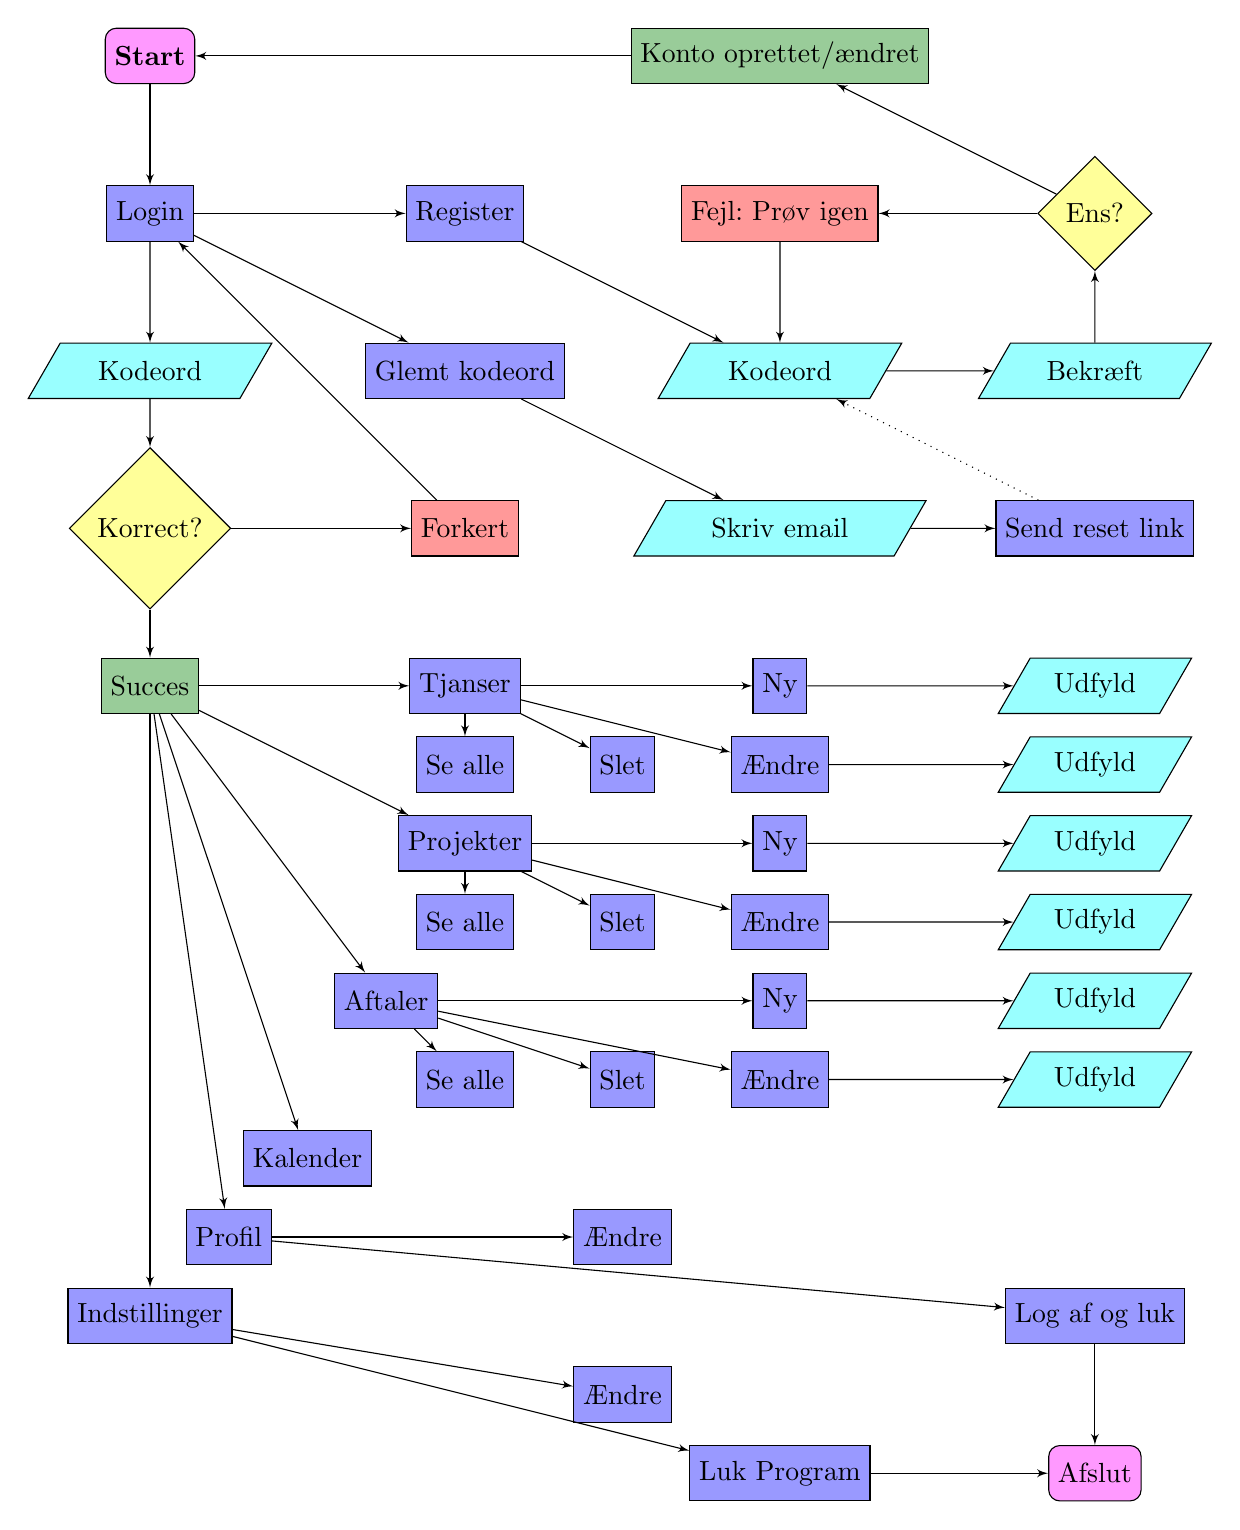
\begin{tikzpicture}

\node[terminator] at (0,0) (start) {\textbf{Start}};

\node[process] at (0,-2) (haveLogin) {Login};

\node[process] at (4,-2) (signUp) {Register};
\node[input] at (8,-4) (inputPass) {Kodeord};
\node[input] at (12,-4) (confirmPass) {Bekræft};
\node[decision] at (12,-2) (matchPass) {Ens?};
\node[positive] at (8,0) (createAcc) {Konto oprettet/ændret};
\node[negative] at (8,-2) (passAgain) {Fejl: Prøv igen};


\node[input] at (0,-4) (havePass) {Kodeord};
\node[process] at (4,-4) (forgottenPass) {Glemt kodeord};
\node[input] at (8,-6) (resetPassEmail) {Skriv email};
\node[process] at (12,-6) (resetPassSent) {Send reset link};

\node[decision] at (0,-6) (passCorrect) {Korrect?};
\node[negative] at (4,-6) (passCorrectNo) {Forkert};
\node[positive] at (0,-8) (passCorrectYes) {Succes};

\node[process] at (4,-8) (chores) {Tjanser};
\node[process] at (8,-8) (choresCreate) {Ny};
\node[input] at (12,-8) (choresCreateInput) {Udfyld};
\node[process] at (8,-9) (choresChange) {Ændre};
\node[input] at (12,-9) (choresChangeInput) {Udfyld};
\node[process] at (4,-9) (choresView) {Se alle};
\node[process] at (6,-9) (choresDelete) {Slet};

\path [connector] (chores) -- (choresCreate);
\path [connector] (choresCreate) -- (choresCreateInput);
\path [connector] (chores) -- (choresChange);
\path [connector] (choresChange) -- (choresChangeInput);
\path [connector] (chores) -- (choresView);
\path [connector] (chores) -- (choresDelete);


\node[process] at (4,-10) (projects) {Projekter};
\node[process] at (8,-10) (projectsCreate) {Ny};
\node[input] at (12,-10) (projectsCreateInput) {Udfyld};
\node[process] at (8,-11) (projectsChange) {Ændre};
\node[input] at (12,-11) (projectsChangeInput) {Udfyld};
\node[process] at (4,-11) (projectsView) {Se alle};
\node[process] at (6,-11) (projectsDelete) {Slet};

\path [connector] (projects) -- (projectsCreate);
\path [connector] (projectsCreate) -- (projectsCreateInput);
\path [connector] (projects) -- (projectsChange);
\path [connector] (projectsChange) -- (projectsChangeInput);
\path [connector] (projects) -- (projectsView);
\path [connector] (projects) -- (projectsDelete);


\node[process] at (3,-12) (appointments) {Aftaler};
\node[process] at (8,-12) (appointmentsCreate) {Ny};
\node[input] at (12,-12) (appointmentsCreateInput) {Udfyld};
\node[process] at (8,-13) (appointmentsChange) {Ændre};
\node[input] at (12,-13) (appointmentsChangeInput) {Udfyld};
\node[process] at (4,-13) (appointmentsView) {Se alle};
\node[process] at (6,-13) (appointmentsDelete) {Slet};

\path [connector] (appointments) -- (appointmentsCreate);
\path [connector] (appointmentsCreate) -- (appointmentsCreateInput);
\path [connector] (appointments) -- (appointmentsChange);
\path [connector] (appointmentsChange) -- (appointmentsChangeInput);
\path [connector] (appointments) -- (appointmentsView);
\path [connector] (appointments) -- (appointmentsDelete);



\node[process] at (2,-14) (calendar) {Kalender};

\node[process] at (1,-15) (profile) {Profil};
\node[process] at (6,-15) (profileChange) {Ændre};
\node[process] at (12,-16) (profileLogout) {Log af og luk};

\node[process] at (0,-16) (settings) {Indstillinger};
\node[process] at (6, -17) (settingsChange) {Ændre};
\node[process] at (8,-18) (settingsTerm) {Luk Program};

\node[terminator] at (12,-18) (end) {Afslut};

\path [connector] (start) -- (haveLogin);

\path [connector] (haveLogin) -- (signUp);
\path [connector] (signUp) -- (inputPass);
\path [connector] (inputPass) -- (confirmPass);
\path [connector] (confirmPass) -- (matchPass);
\path [connector] (matchPass) -- (createAcc);
\path [connector] (matchPass) -- (passAgain);
\path [connector] (passAgain) -- (inputPass);
\path [connector] (createAcc) -- (start);

\path [connector] (haveLogin) -- (havePass);
\path [connector] (haveLogin) -- (forgottenPass);
\path [connector] (forgottenPass) -- (resetPassEmail);
\path [connector] (resetPassEmail) -- (resetPassSent);
\path [semiConnector] (resetPassSent) -- (inputPass);


\path [connector] (havePass) -- (passCorrect);
\path [connector] (passCorrect) -- (passCorrectNo);
\path [connector] (passCorrectNo) -- (haveLogin);
\path [connector] (passCorrect) -- (passCorrectYes);

\path [connector] (passCorrectYes) -- (chores);
\path [connector] (passCorrectYes) -- (projects);
\path [connector] (passCorrectYes) -- (appointments);
\path [connector] (passCorrectYes) -- (calendar);

\path [connector] (passCorrectYes) -- (profile);
\path [connector] (profile) -- (profileLogout);
\path [connector] (profile) -- (profileChange);
\path [connector] (profileLogout) -- (end);

\path [connector] (passCorrectYes) -- (settings);
\path [connector] (settings) -- (settingsTerm);
\path [connector] (settings) -- (settingsChange);
\path [connector] (settingsTerm) -- (end);




\end{tikzpicture}

\begin{comment}
\node [data] at (0,-2) (data) {Provide data};
\node [decision] at (0,-5) (decision) {Valid data?};
\node [error] at (3.5,-5) (error) {Error};
\node [success] at (0,-8) (success) {Success};
\node [terminator] at (0,-10) (end) {\textbf{End}};
\node[draw=none] at (1.85, -4.75) (no) {No};
\node[draw=none] at (0.35, -6.75) (yes) {Yes};



\path [connector] (start) -- (data);
\path [connector] (data) -- (decision);
\path [connector] (decision) -- (error);
\path [connector] (decision) -- (success);
\path [connector] (error) |- (end);
\path [connector] (success) -- (end);
\end{comment}


\end{center}

\section{Mockup}
\label{mockup}

Jeg har valgt at inkludere 6 skærme i denne mock-up. Kun 3 er en del af kernen opgaven og derfor har jeg fokuseret på dem. Ville har dog indkluderet de 3 ekstra faner, Kalender-, Profil- og Indstillingsfanen, fordi jeg på den ene side håber at kunne nå dem og for at vise, at der tænkt yderligere menuer ind. Jeg vil dog koncentrere mig tid på de 3 vigtigste faner.\par{}
Billedet af en tablet er fundet her\footnote{https://purepng.com/photo/25263/electronics-android-tablet}. Farverne har jeg valgt en tertiære farve, som jeg kunne lide og brugte \textit{colorhex.com} til at finde dens triadiske farveskema\footnote{https://www.colorhexa.com/ff99ff}. Jeg valgte et triadisk farveskema, fordi det både er farverigt og udtryksfuld, men stadig harmoniserende\footnote{https://multimediedesigneren.dk/farveteori-og-farvehjul/}. Det bliver dog ikke endelige farvevalg, da dette specifikke triadiske farveskema ikke er så harmoniserende.\footnote{Bortset fra centsors version af programmet, som ikke har mulighed for at skifte farveskemaet}.\par{}
Jeg har ikke lavet et flowchart, men i stedet for at forsøgt at forklare det her.\par{}

\pic[jpg]{mockUpTjans}
Her viser programmet de top 5 vigtigste Tjanser. Tjanser er tilbagevendende og har beskrivelse, en nuværende eller kommende tilstand, et interval og en prioritet.
\begin{itemize}
\item \textbf{Lav ny} lader dig oprette en tjans.
\item \textbf{Se alle} viser alle nuværende tjanser og ikke kun de 5 højest prioriterede.
\item \textbf{Kommende} viser alle kommende tjanser
\item Tjanserne er de vigtigste interaktioner og der kan man trykke flere forskellige steder på knappen:
\begin{itemize}
\item \textbf{I midten} viser beskrivelse ad tjansen og mulighed for at kunne ændre tjansens indstillinger.
\item \textbf{Venstre side}: sætter tjansen til kommende for dens intervallet og øger dens prioritet.
\item \textbf{Højre side}: sætter tjansen til kommende for dens intervallet og dens prioritet til, hvad den var da den oprettes.
\item Når knapperne bliver smalle nok, forsvinder først den venstre knap og derefter den højre. I de ville kunne tilgås ved at trykke \textbf{i midten}.
\end{itemize}
\end{itemize}

\pic[jpg]{mockUpProjekt}
Her vises de 5 aktive projekter med den seneste aktivitet. Projekter har blot en beskrivelse, aktiv eller passiv tilstand; og en fremskridtstræller.
\begin{itemize}
\item \textbf{Ny}: Opretter en nyt projekt.
\item \textbf{Aktive} viser alle aktive projekter og ikke kun de 5 med seneste aktivitet.
\item \textbf{Passive} viser alle passive projekter.
\item Projekter er de vigtigste interaktioner og der kan man trykke flere forskellige steder på knappen:
\begin{itemize}
\item \textbf{I midten} viser beskrivelse af projektet, dets fremskridt, mulighed for at ændre dens indstilliger eller nulstille dens fremskridt.
\item \textbf{Venstre side}: sætter projektet til passiv.
\item \textbf{Højre side}: sætter projektets en højere.
\item Når knapperne bliver smalle nok, forsvinder først den venstre knap og derefter den højre. I de ville kunne tilgås ved at trykke \textbf{i midten}.
\end{itemize}
\end{itemize}

\pic[jpg]{mockUpAftale}
Her vises de 5 næste relevante alle. Aftaler har en beskrivelse, relevans-status, tidspunkt og indstillinger for påmindelser.
\begin{itemize}
\item \textbf{Ny}: Opretter en ny aftale..
\item \textbf{Se alle} viser alle kommende aftaler og ikke kun de 5 næste.
\item \textbf{Tidligere} viser alle tidligere aftaler samt kommende ikke-relevante aftaler.
\item Aftaler er de vigtigste interaktioner og der kan man trykke flere forskellige steder på knappen:
\begin{itemize}
\item \textbf{I midten} viser beskrivelse af aftalen og får mulighed for at ændre dens indstilliger-
\item \textbf{Venstre side}: mulighed for at ændre dens tidspunkt eller påmindelse.
\item \textbf{Højre side}: sætte aftalen til ikke-relevante.
\item Når knapperne bliver smalle nok, forsvinder først den venstre knap og derefter den højre. I de ville kunne tilgås ved at trykke \textbf{i midten}.
\end{itemize}
\end{itemize}

\pic[jpg]{mockUpKalender}
Viser en, endnu ikke desginet, kalender, hvor man kan se ens aktivitet. De forskellige opgaver vises lidt forskellige. Der ville også skulle være en række styringsknapper.\par{}
Aftales tidspunkter vises samt hvornår aftaler ikke længere relevante, om det så skyldes om man færdiggjorde dem før tid eller de blot oprendte, gøres der ikke forskel på.\par{}
For projekter vises der, hver gang man har trykket fremskridt for et projekt.\par{}
For tjanser vises der hver gang en sættes til kommende, uanset om den har ændret prioritet.

\pic[jpg]{mockUpProfil}
Her vises, en endnu udesignet, profilfane, hvor det vil være muligt at få et overblik over ens profil og ændre den.

\pic[jpg]{mockUpIndstillinger}
Her vises, en endnu udesignet, indstillingsfane, hvor det vil være muligt at styre en række ting fra. Eksempelvis antallet af tjanser, aftaler og projekter eller lignende ting.

\chapter{Teknisk dokumentation}

\section{Få programmeret til at køre}

Indtil videre er det nødvendigt bruge \fragCom{uvicorn main:app --reload} fra \textit{./API/}-mappen for at få backenden til at køre og bruge \fragCom{npm run web} eller \fragCom{npm run webnb}\footnote{hvis man ikke ønsker applikationen selv skal åbne sig i en ny browser} fra \textit{./UI/}-mappen for at få fronten til at køre.\par{}
Backenden virker som den skal, men frontenenden fejler desværre på en centralskærm.\par{}

Jeg håber på at udbedre dette og lave en ny vejledning\par{}

\section{Testkonditioner}

Det er muligt at logge ind, lave en bruger og anmode om at få en reset password token fra fronten i skrivende tidspunkt.\par{}
Det er ikke imponerende, men det betyder, at de fleste frontend test ikke giver mening.
Jeg har dog testet alle end points.\par{}

\section{Testede API routes}

Disse routes er testet fra localhost:

\begin{table}[H]
\centering
\rowcolors{2}{White}{Gray!25}
\begin{tabularx}{\textwidth}{X X X}

[HTTP request metoden] /[route]
&
funktion
&
Test 8/12
\\


GET	/
&
Root
&
\textcolor{ForestGreen}{succes!}
\\


GET	/authticated-route
&
Authenticated Route
&
\textcolor{ForestGreen}{succes!}
\\

GET /status
&
Getstatus
&
\textcolor{Bittersweet}{Fejlet!}
\\


POST /auth/jwt/login
&
Auth:Jwt.Login
&
\textcolor{ForestGreen}{succes!}
\\

POST /auth/jwt/logout
&
Auth:Jwt.Logout
&
\textcolor{ForestGreen}{succes!}
\\

POST /auth/register
&
Register:Register
&
\textcolor{ForestGreen}{succes!}
\\

POST /auth/forgot-password
&
Reset:Forgot Password
&
\textcolor{ForestGreen}{succes!}
\\

POST /auth/reset-password
&
Reset:Reset Password
&
\textcolor{ForestGreen}{succes!}
\\

POST /auth/request-verify-token
&
Verify:Request-Token
&
\textcolor{ForestGreen}{succes!}
\\

POST /auth/verify
&
Verify:Verify
&
\textcolor{ForestGreen}{succes!}
\\

GET /users/me
&
Users:Current User
&
\textcolor{ForestGreen}{succes!}
\\

PATCH /users/me
&
Users:Patch Current User
&
\textcolor{ForestGreen}{succes!}
\\

GET /users/{id}
&
Users:User
&
\textcolor{ForestGreen}{succes!}
\\

DELETE /users/{id}
&
Users:Delete User
&
\textcolor{ForestGreen}{succes!}
\\

PATCH /users/{id}
&
Users:Patch User
&
\textcolor{ForestGreen}{succes!}
\\

GET /appointments/
&
Routetosomething
&
\textcolor{ForestGreen}{succes!}
\\

POST /appointments/
&
Routetocreation
&
\textcolor{ForestGreen}{succes!}
\\

GET /appointments/{id}
&
Routetoonething
&
\textcolor{ForestGreen}{succes!}
\\

PUT /appointments/{id}
&
Routetoupdate
&
\textcolor{ForestGreen}{succes!}
\\

DELETE /appointments/{id}
&
Routetooblivion
&
\textcolor{ForestGreen}{succes!}
\\

\hline
\end{tabularx}
\end{table}

\begin{table}[H]
\centering
\rowcolors{2}{White}{Gray!25}
\begin{tabularx}{\textwidth}{X X X}

[HTTP request metoden] /[route]
&
funktion
&
Test 8/12
\\

GET /chores/
&
Routetosomething
&
\textcolor{ForestGreen}{succes!}
\\

POST /chores/
&
Routetocreation
&
\textcolor{ForestGreen}{succes!}
\\

GET /chores/{id}
&
Routetoonething
&
\textcolor{ForestGreen}{succes!}
\\

PUT /chores/{id}
&
Routetoupdate
&
\textcolor{ForestGreen}{succes!}
\\

DELETE /chores/{id}
&
Routetooblivion
&
\textcolor{ForestGreen}{succes!}
\\



GET /projects/
&
Routetosomething
&
\textcolor{ForestGreen}{succes!}
\\

POST /projects/
&
Routetocreation
&
\textcolor{ForestGreen}{succes!}
\\

GET /projects/{id}
&
Routetoonething
&
\textcolor{ForestGreen}{succes!}
\\

PUT /projects/{id}
&
Routetoupdate
&
\textcolor{ForestGreen}{succes!}
\\

DELETE /projects/{id}
&
Routetooblivion
&
\textcolor{ForestGreen}{succes!}
\\

GET /tasks/
&
Routetoeverything
&
\textcolor{ForestGreen}{succes!}
\\

POST /tasks/
&
Routetocreation
&
\textcolor{ForestGreen}{succes!}
\\

GET /tasks/{id}
&
Routetoonething
&
\textcolor{ForestGreen}{succes!}
\\

PUT /tasks/{id}
&
Routetoupdate
&
\textcolor{ForestGreen}{succes!}
\\

DELETE /tasks/{id}
&
Routetooblivion
&
\textcolor{ForestGreen}{succes!}
\\

\hline
\end{tabularx}
\end{table}

\subsection{evaluering af fejlet GET /status}
Route fejlede, da den ved en fejl var sat til at kræve autorisering. Det er ikke meningen, så derfor tæller det selvfølgelig som en fejl, selvom det er rettet nu.

\clearpage

\pagenumbering{Roman}
\appendix
\renewcommand{\thechapter}{\Alph{chapter}}

%%%%%%
%	Afslutning
%%%%%%
	
\end{document}
